\section{Experiments}
\label{Sec:Experiments}

This section evaluate Cerberus by answering several key questions.
\begin{itemize}
        \item \textbf{Q1}: will Cerberus improve application performance
                by utilizing burst buffer nodes?
        \item \textbf{Q2}: Will job demand on burst buffer affect Cerberus?
                Why bother to divide the job execution into 3 phases?
        \item \textbf{Q3}: Can dynamic programming based optimization
                help Cerberus further
improve application performance?
\end{itemize}
Our newly developed event-driven simulator, BBSim, is used to simulating
the Trinity system described later.
% metric

We select 2 key evaluation metrics, job's \textit{response time} and 
\textit{system throughput}, when evaluating our design.
Response time is the time duration from job submission to its fully completion,
which is the major concern from user's perspective.
On the other hands, system throughput, defined as the number of jobs finished in
a fixed time period (500 seconds), measures the performance of computing system.

\subsection{Simulation Settings}
% system
We consider simulating the full Trinity super computer\cite{TrinitySystem}.
The number of compute nodes on Trinity is about 18,936,
e.g. 9,436 Intel Haswell nodes
and at least 9500 Intel Xeon Phi nodes.
There are 16 cores on each processor, thus totally 302,976 cores.
In the following experiments, we compare two identical system except that
IO nodes are replaced by the same number of burst buffer nodes.
Eventually Trinity plans to delivery up to 576 burst buffer nodes of 3.7 PB,
consisted of Trinity IO nodes with PCIe SSD card.
They are globally accessible as intermediate storage and distributed among cabinets.
Sequential read/write speed of burst buffer nodes is 8.0 GBps.
Bandwidth between CPU node and non-burst-buffer IO node is set to 2.5 GBps.

% trace
Job trace is from ANL's Blue Gene Intrepid system,
containing totally 68,936 jobs run during January to September 2009\cite{JobTrace}.
We extract two critical fields from this jobs trace: running time and
number of cores user requested.
In this section we take a window of 1,185 jobs and report their scheduling results.
We patched 3 fields to each job's log entry: the amount of input data $data\_in$,
the total amount of written data for checkpointings $data\_run$
and the amount of output data $data\_out$.
We assume $data\_run$ and $data\_out$ follows uniform distribution with
lower boundary of 1 TiB and upper boundary of 60 TiB;
$data\_in$ follows uniform distribution between 1 GiB and 30 Gib.
The patches 3 fields may or may not be used in scheduling,
depends on both the model of the jobs and the experiment scenario.


\subsection{Q1: Cerberus vs. 1-Phase Batch Scheduler}
\label{Sec:Sim:DirectIOvsBB}
In this section, we demonstrate that by utilizing burst buffer nodes,
job scheduler could improve the performance of both applications and system.
We compare two systems:
\begin{itemize}
        \item \textbf{1-Phase IO}: system without burst buffer nodes
                scheduled by FCFS policy
        \item \textbf{Cerberus}: system with burst buffer 
                scheduled by our proposed Cerberus
\end{itemize}

Figure~\ref{Fig:DirectIOvsBBResponse} compares CDF of the response time of 1185 jobs.
When scheduler can allocate burst buffer to jobs,
response time is bounded by 376,443.12 seconds.
However, the worst case in system without burst buffer
(1-Phase IO) is catastrophical.
There are jobs that takes 889,239.20 seconds to finish,
which is 2.36 times slow as the most non-responsive job
in system equipped with burst buffer.
In average case, \textit{nearly 99\% of the jobs scheduled by Cerberus
response faster than 1-Phase batch scheduler on non-BB system.}
The improvement mainly comes from the difference of IO operation efficiency between
traditional IO nodes and burst buffer nodes.

Figure~\ref{Fig:DirectIOvsBBWait} reveals the total waiting time for both cases.
Notice that system without burst buffer only request compute nodes.
In this case, waiting time is the duration from its submission
to actual starting running.
The difference of worst case waiting time is drastic.
Without burst buffer nodes, job's wait duration in worst case is 3.02 times
slow as the worst one on systems with burst buffer;
the upper bound of waiting duration for burst buffer systems is about 285,254 seconds.
Because of burst buffer's better ability to
absorb checkpoint operations and data moving in/out,
the execution pipeline of job series is significantly speed up.
Statistically, \textit{more than 80\% jobs waited less time, thus response faster,
if they can access burst buffer.}


Using the collected completion time, we calculate system's throughput over time sequence.
Figure~\ref{Fig:DirectIOvsBBThroughput} shows the system throughput for
both system using burst buffer nodes and not.
As indicated by the bar chart,
\textit{the ratio of average throughput between two systems is 2.36},
namely 1.575 to 0.667.
It totally takes 889,239 seconds for the system without burst buffer nodes to
server all 1185 jobs.
The last job is job \#1150, which requested 4096 cores and 59 TB data space.
It starts at 1126 seconds but waited 827,241 seconds.
In contrast, when system installed burst buffer nodes,
it accomplishes the same 1185 jobs in 376,443 seconds.
Job \#1150 is the second last job finished, but both its waiting time and response time
are significantly reduced, 272,741 and 376,026 seconds respectively.

\begin{figure*}[!t]
        \centering
        \subfloat[Job Response Time] {
                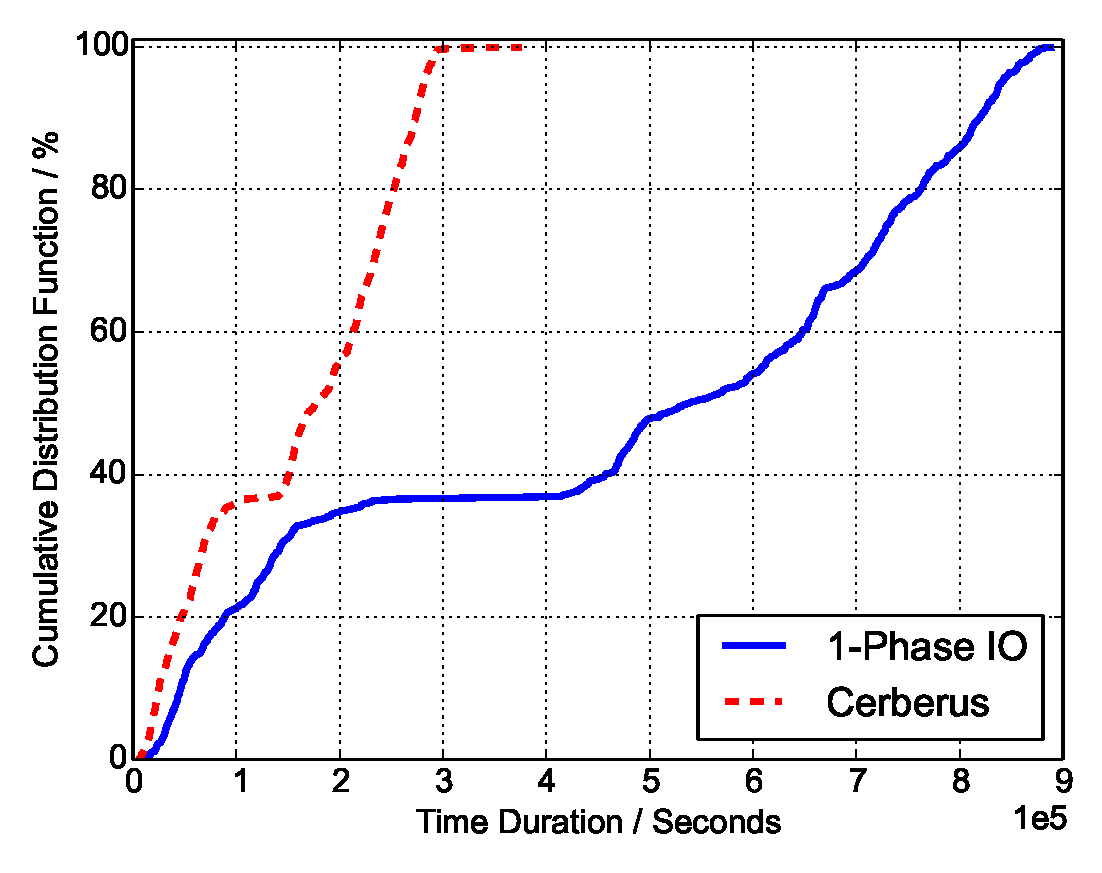
\includegraphics[width=3.2in]{IOvsBBFigures/1000jobs_direct_vs_bb_response}
                \label{Fig:DirectIOvsBBResponse}
        }
        ~
        \subfloat[Job Wait Time] {
                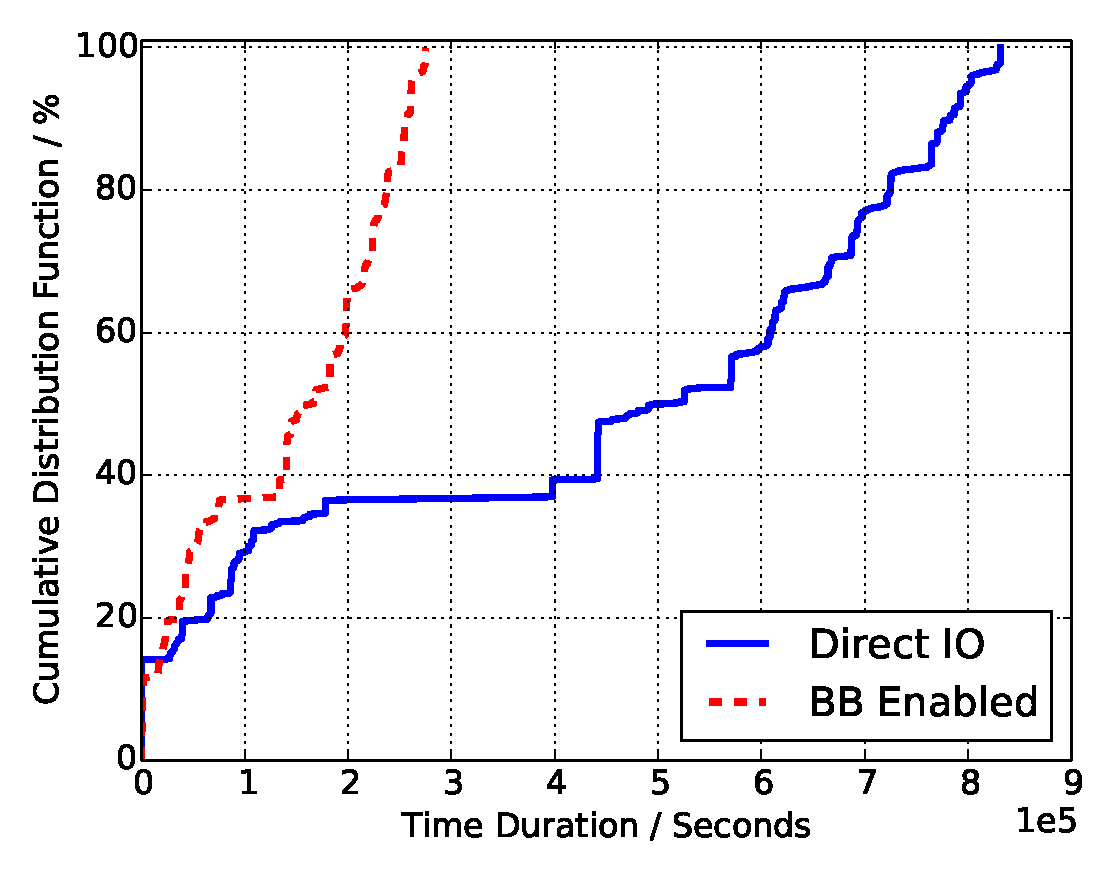
\includegraphics[width=3.2in]{IOvsBBFigures/1000jobs_direct_vs_bb_wait}
                \label{Fig:DirectIOvsBBWait}
        }
        \caption{Performance of 1185 Applications: IO Node Only System vs. Burst Buffer System}
        \label{Fig:DirectIOPerformance}
\end{figure*}

\begin{figure}[!t]
        \centering
        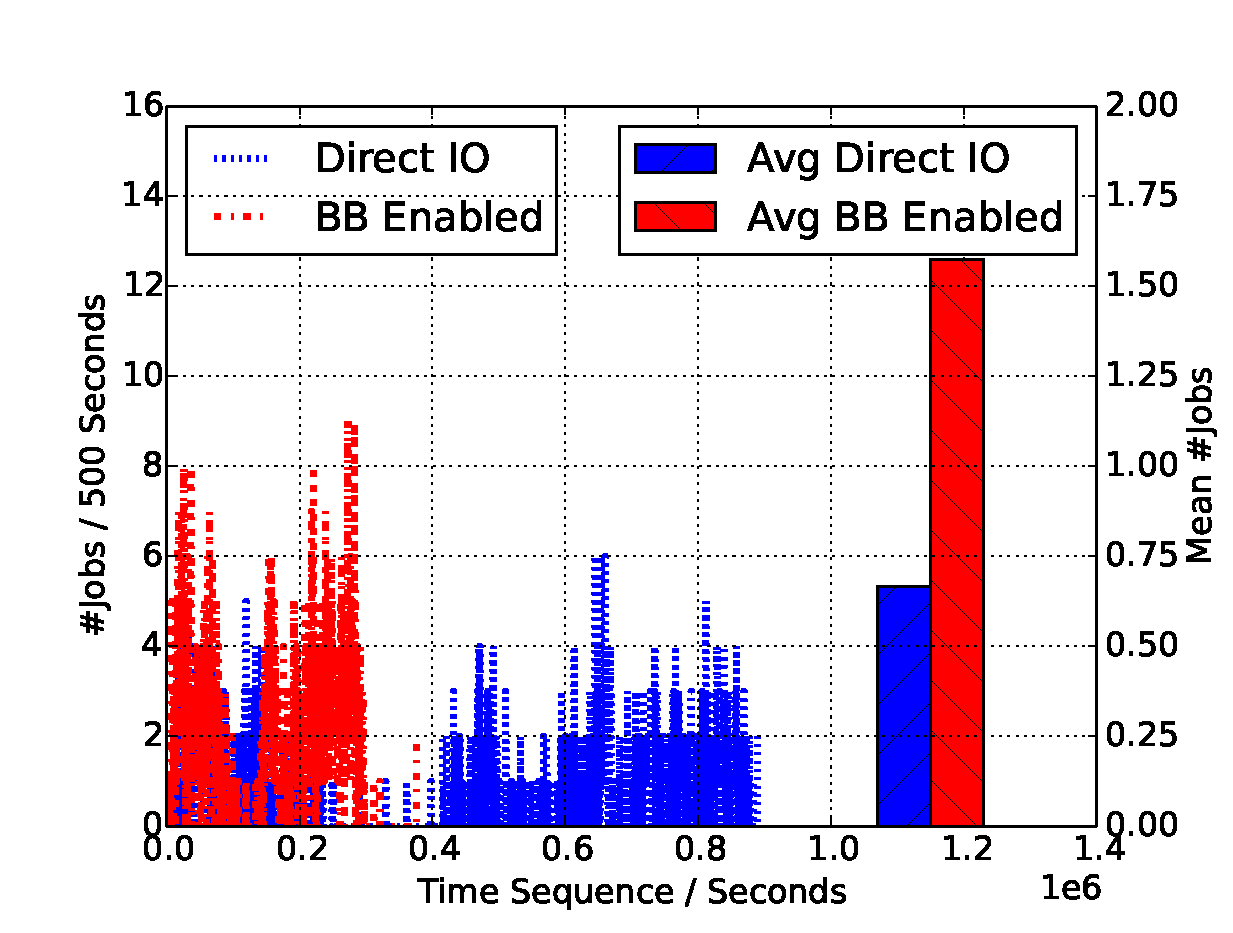
\includegraphics[width=3.2in]{IOvsBBFigures/1000jobs_direct_vs_bb_throughput}
        \caption{System Throughput, IO Node Only vs. Burst Buffer System}
        \label{Fig:DirectIOvsBBThroughput}
\end{figure}


\subsection{Q2: Demand Granularity Matters?}
In this section we validate our 3-phase model.
Applications are benefited when scheduler dividing jobs into 3 separated phases and 
scheduling are based on corresponding burst buffer demand in each phase.
This suggests that user should provide burst buffer demand as granular as possible.

In Figure~\ref{Fig:3Pvs1PResponse}, we plot 3 different scheduling results by 3 FCFS scheduler.
\begin{itemize}
        \item \textbf{1-Phase BB}: Jobs are modeled as just 1 phase.
                Users just provide general burst buffer demand throughout
                entire application lifetime.
        \item \textbf{1D Cerberus}: In this case Cerberus only knows
                the overall burst buffer demand.
        \item \textbf{Cerberus}: Users kindly provided all the burst buffer
                demand in all 3 phases.
                %the same as Cerberus in section~\ref{Sec:Sim:DirectIOvsBB}
\end{itemize}
We simulate the 3 cases with the same generated random data volume sequence.
We assume the overall burst buffer demand in 1-phase BB and 1D Cerberus is
$\max \{data\_in, data\_out, data\_run\}$.
Notice that 1-phase BB scheduler must subject to burst buffer capacity constraint.
%For 1-phase-modeled jobs, scheduler will make decision
%based on $\max \{data\_in, data\_out, data\_run\}$
%since we assume user will only tell the upper bound of its application's demand.
%However, in simulation, we use the generated data amount as the same as 3-modeled jobs.
%Response time of system without burst buffer devices are also plotted for comparison.

%Unsurprisingly, jobs' response time is improving as long as they could utilizing burst buffer.
When comparing scheduling results of 1-Phase BB and 1D Cerberus,
both of which only have rough data information of application,
more than 60\% of the 3-phase-modeled jobs finish faster than 1-phase-modeled jobs.
The longest 3-phase-modeled job takes 418,927 seconds to finish
while the slowest 1-phase-modeled job needs about 492,591 seconds to finish.
The improvement is about 14.95\% for the worst case.
The reason of such improvement is as follows.
For the 1-phase-modeled jobs, burst buffer nodes will be exclusively
taken by scheduled jobs throughout their lifetime.
In contrast, Cerberus will reclaim burst buffer multiple times;
it also releases burst buffer nodes and CPU resources as soon as possible.
This gives Cerberus more opportunity to schedule the system resources.
At last, when comparing the case of Cerberus with 1D Cerberus,
we find another advantage of our 3-phase model.
If benign users can provide finer-grain information of data/IO demand,
Cerberus can programme each queue separately and get better scheduling result.
In our simulation,
since Cerberus knows more about application's demand in different phases,
the worst absolute response time is less than 379,026 seconds.
This is 10.24\% improvement to 3-phase-modeled jobs
when Cerberus only knows the upper bound of data demand,
23.66\% better than the slowest 1-phase-modeled job.
In average case, \textit{more than 80\% of the jobs 
scheduled by Cerberus finish earlier than 1-phase-modeled jobs.}
Meanwhile, \textit{more than 60\% of the jobs takes less time if user 
specifies data usage demand at each phase to Cerberus, e.g. Cerberus vs. 1D Cerberus.}

We can reason about why Cerberus's scheduling result is better than
naively integrating batch scheduler with burst buffer constraint
by looking at the detailed waiting time.
Figure~\ref{Fig:3Pvs1PWaitRun} shows the time job spend in running queue.
There are 3 queues in Cerberus;
correspondingly we have 3 kinds of waiting for jobs in Cerberus.
%Figure~\ref{Fig:3Pvs1PWaitIn} shows the time job spend in inputing queue,
%Figure~\ref{Fig:3Pvs1PWaitOut} the time job spend in outputing queue.
For 1-phase-modeled jobs, there is just one queue;
therefore the waiting time in Figure~\ref{Fig:3Pvs1PWaitRun} is the total waiting time.
We see that jobs did not spend much time in either input queue $Q_I$ or output queue.
The upper bounds of time spent in input queue are
2500 seconds for 1D Cerberus and Cerberus respectively.
This is because input data is very small (tens of GB level)
comparing to checkpointing data and application output (tens of TB level).
In contrast, in worst case job scheduled by 1-Phase BB needs to wait for 443,203 seconds,
because scheduler makes one-time decision on the basis of demand of
both computer node and maximum burst buffer.
%the upper bounds of time spent in output queue $Q_O$ are
%less than 5\% of the total waiting time of 1-phase-scheduler case
%for both 3-phases cases.
As for the time waiting for running, more than 60\% of the jobs scheduled by
1D Cerberus and Cerberus are better than 1-phase-modeled jobs.
The difference of waiting time results in the different
response performance.

Figure~\ref{Fig:3Pvs1PThroughput} describes system throughput of these three different scenarios.
It helps us examine the performance of the scheduling in time sequence.
For 1-phase-modeled job, we can see an obvious `throughput gap'
from 150,000 second to 200,000 second approximately,
similar for the case of 1D Cerberus, throughput also starts provocatively,
Cerberus' runs counter to both previous cases.
Even though there is a throughput trough between 100,000 to 150,000 seconds,
Cerberus manages to make the system having high throughput at the beginning and
later (from 150,000 to 300,000 seconds).
\textit{In average, the throughput of Cerberus is 1.575 jobs / 500 seconds.}
It is 11.39\% of the 1-Phase BB case (1.414 jobs / 500 seconds) and
31.03\% higher than the 1D Cerberus case (1.202 jobs / 500 seconds).
We believe this validates the indispensable 3 phase job model and
the necessity that user provides data capacity demand for each phase.


\begin{figure*}[!t]
        \centering
        \subfloat[Job Response Time] {
                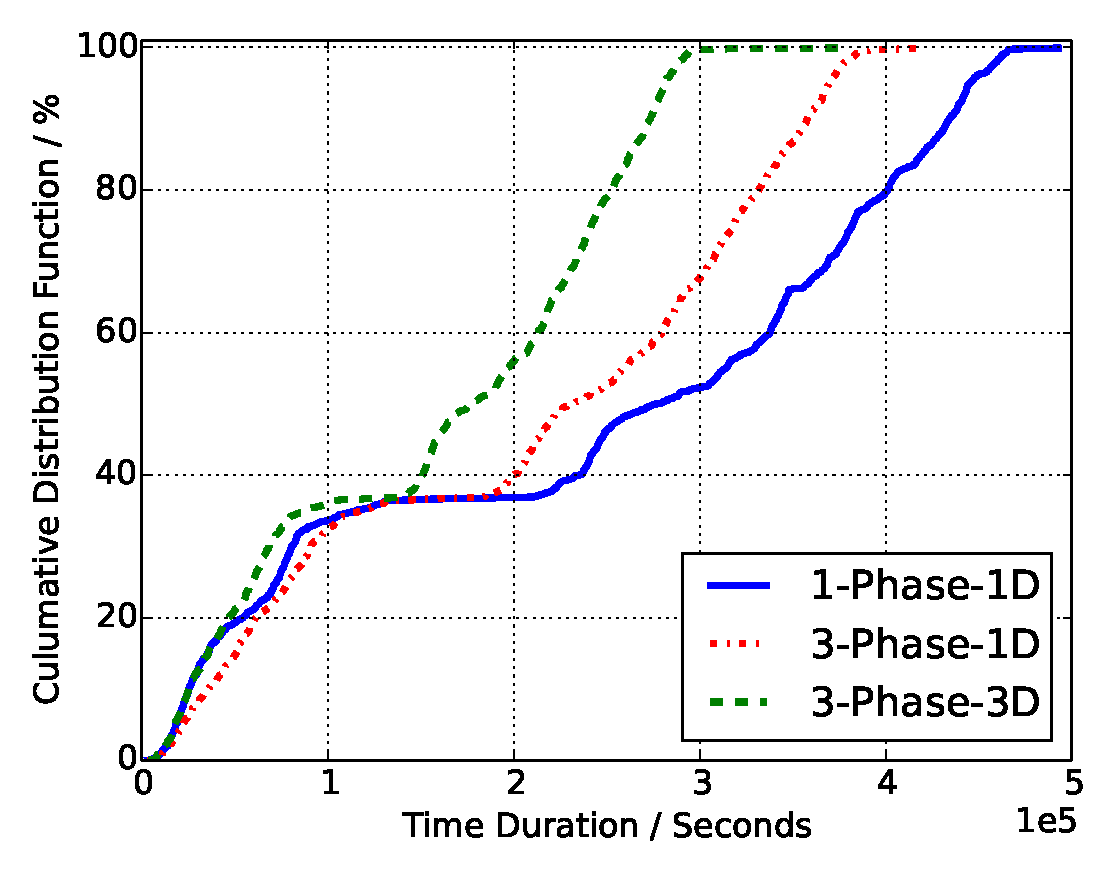
\includegraphics[width=3.2in]{3Pvs1PFigures/1000jobs_3p_vs_1p_response}
                \label{Fig:3Pvs1PResponse}
        }
        ~
        %\subfloat[Job Wait Time] {
                %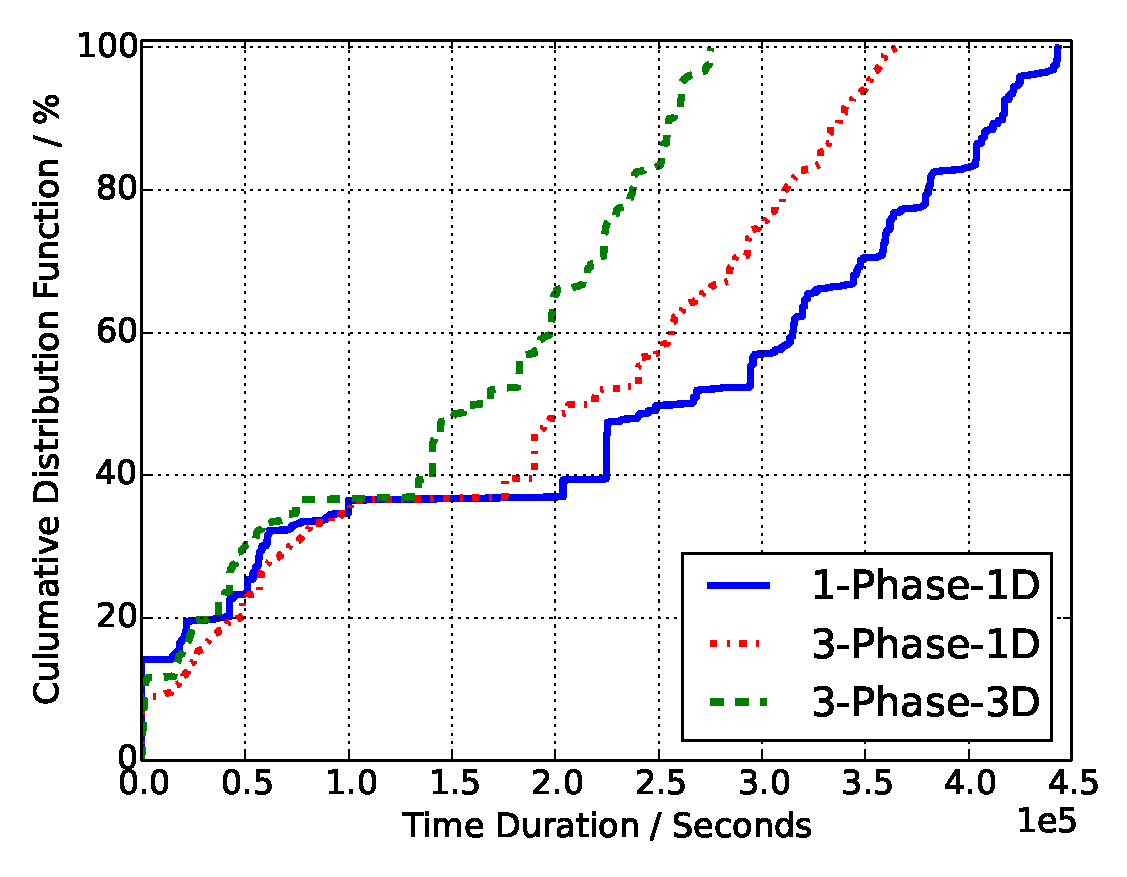
\includegraphics[width=3.2in]{3Pvs1PFigures/1000jobs_3p_vs_1p_wait}
                %\label{Fig:3Pvs1PWait}
        %}
        %\subfloat[Job Wait Input Time] {
                %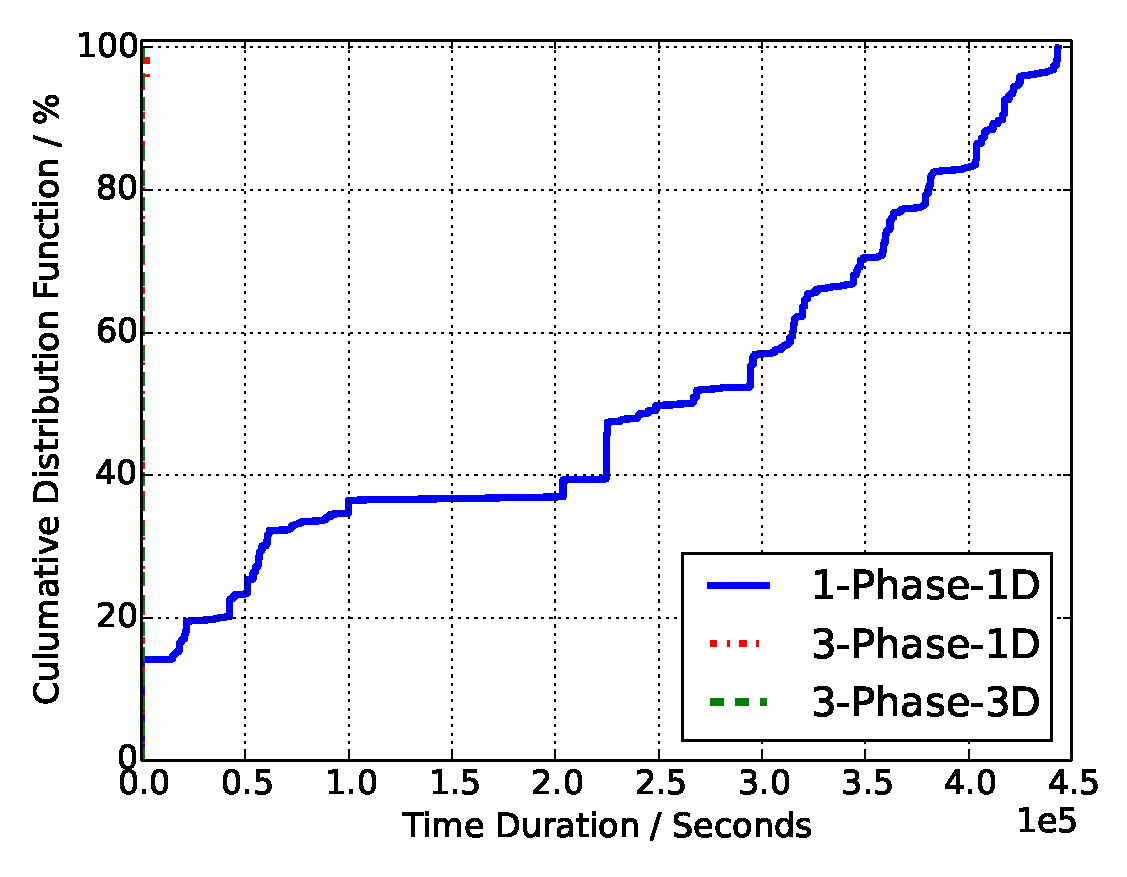
\includegraphics[width=2.3in]{3Pvs1PFigures/1000jobs_3p_vs_1p_wait_in}
                %\label{Fig:3Pvs1PWaitIn}
        %}
        %~
        \subfloat[Job Wait Run Time] {
                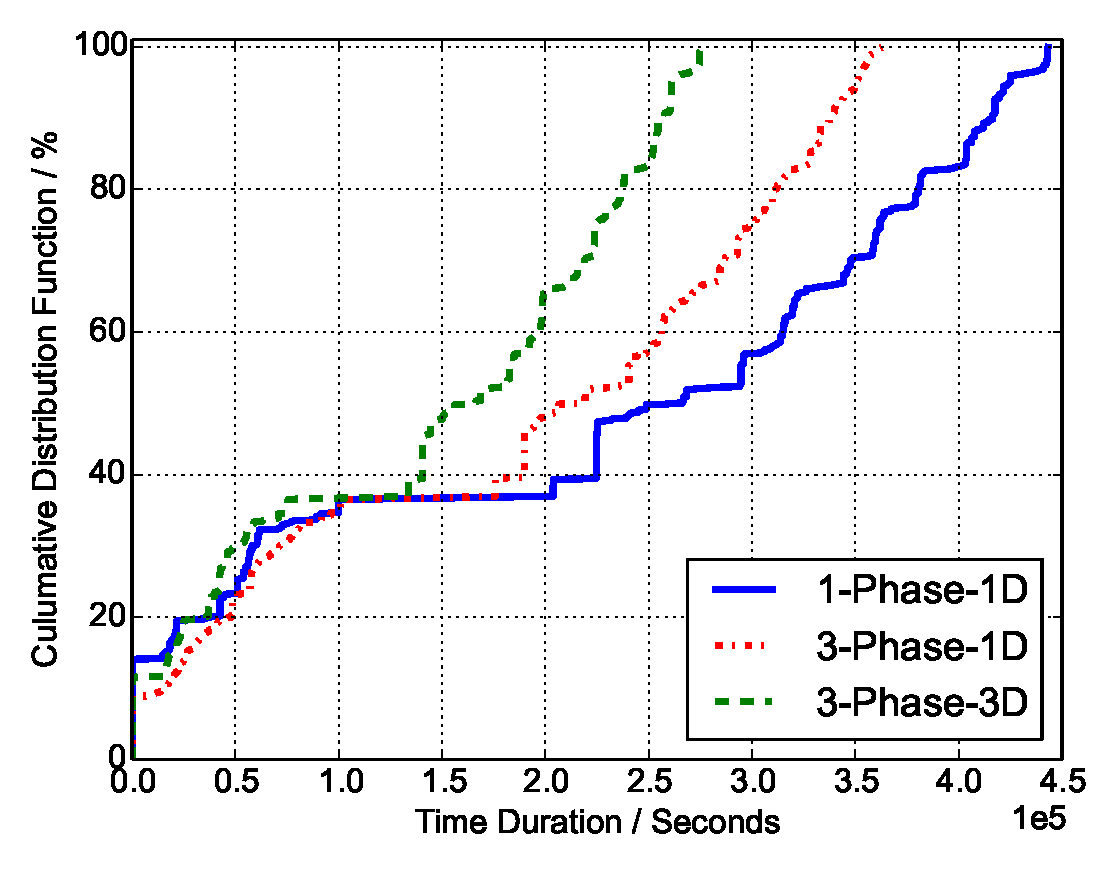
\includegraphics[width=3.2in]{3Pvs1PFigures/1000jobs_3p_vs_1p_wait_run}
                \label{Fig:3Pvs1PWaitRun}
        }
        ~
        %\subfloat[Job Wait Output Time] {
                %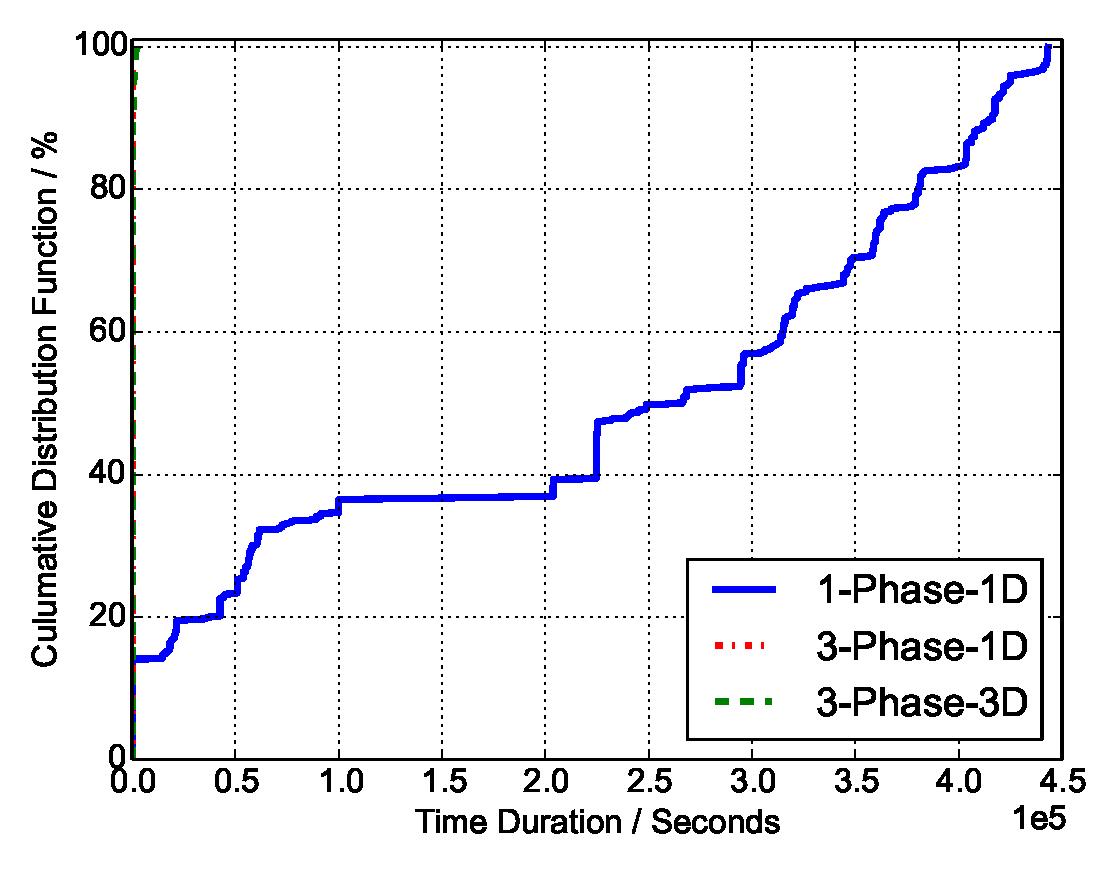
\includegraphics[width=2.3in]{3Pvs1PFigures/1000jobs_3p_vs_1p_wait_out}
                %\label{Fig:3Pvs1PWaitOut}
        %}
        \caption{Performance of 1185 Applications: 1 Phase Model vs. 3 Phase Model}
        \label{Fig:3Pvs1PPerformance}
\end{figure*}

\begin{figure*}[!t]
        \centering
        \subfloat[Job Response Time] {
                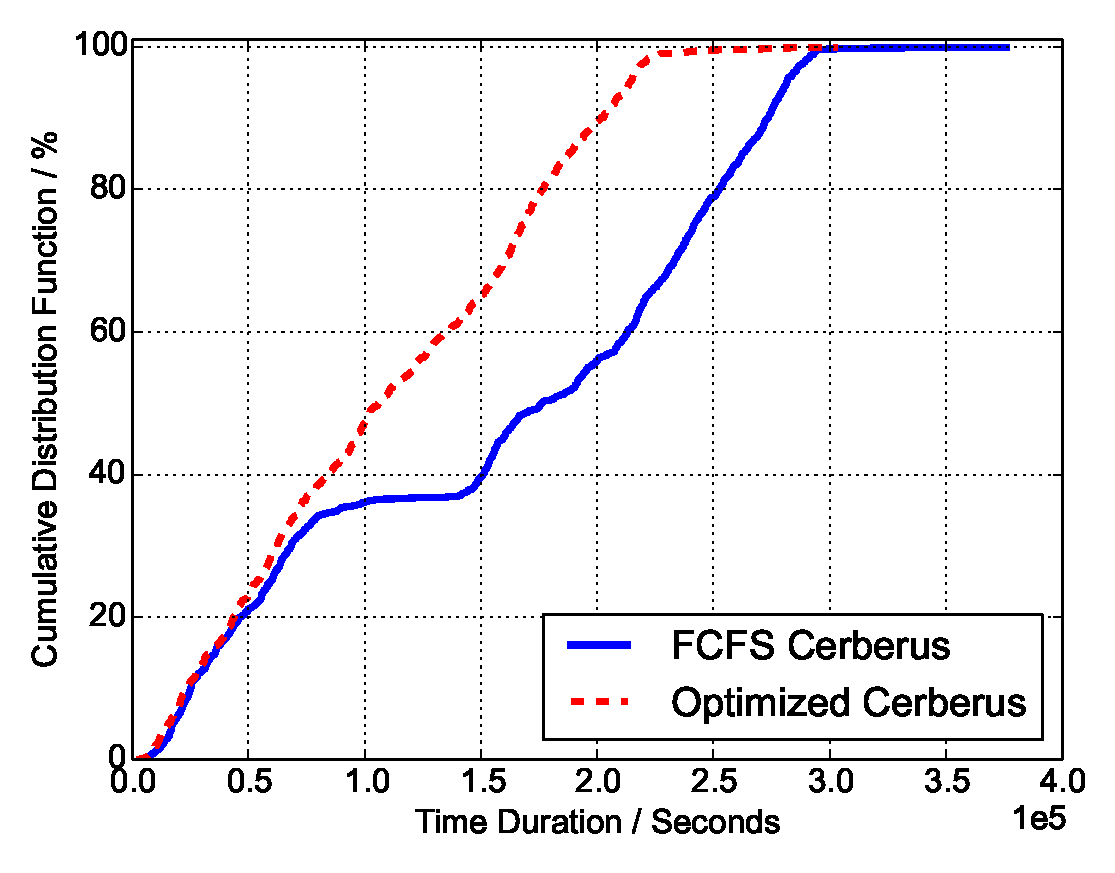
\includegraphics[width=3.2in]{DPvsFIFOFigures/1000jobs_dp_vs_fifo_response}
                \label{Fig:DPvsFIFOResponse}
        }
        ~
        \subfloat[Job Wait Run Time] {
                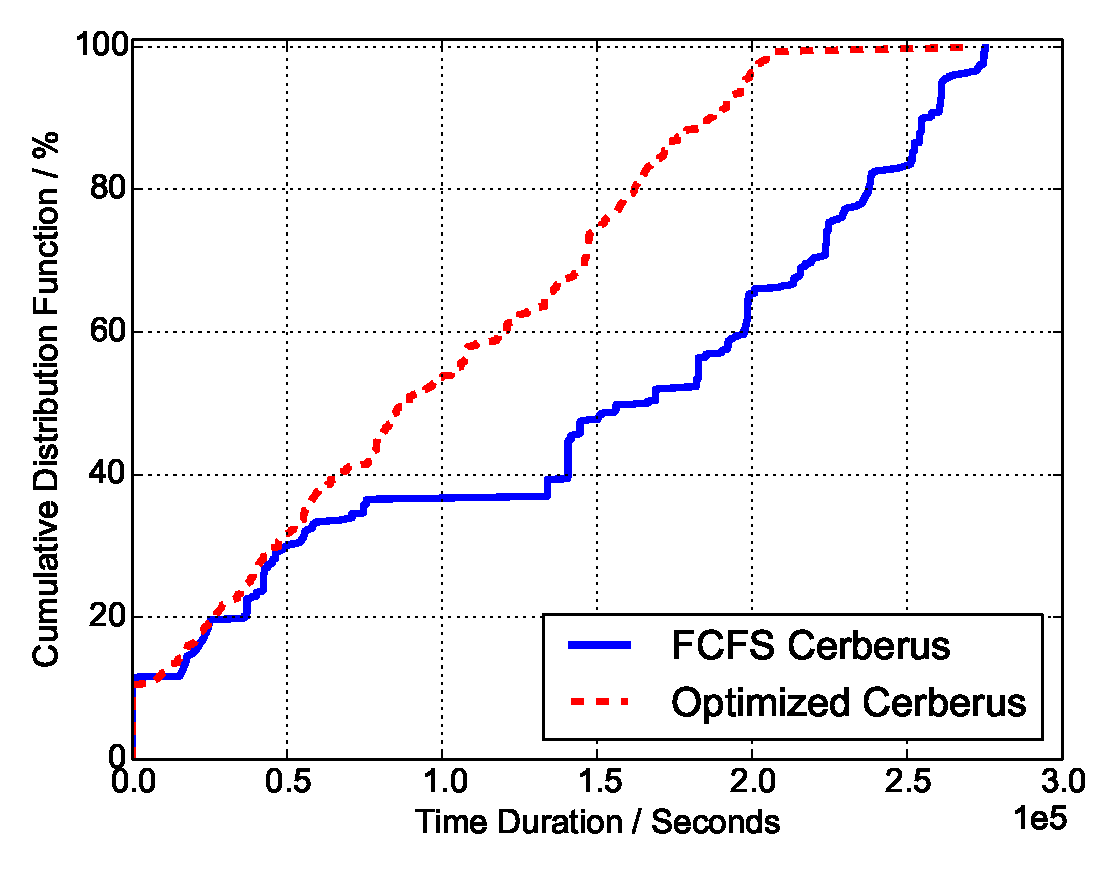
\includegraphics[width=3.2in]{DPvsFIFOFigures/1000jobs_dp_vs_fifo_wait_run}
                \label{Fig:DPvsFIFOWaitRun}
        }
        \caption{Performance of 1185 Applications: Optimized Cerberus vs. FCFS Cerberus}
        \label{Fig:DPvsFIFOPerformance}
\end{figure*}


\subsection{Q3: Cerberus vs. Optimized Cerberus}
If we consider optimizing either burst buffer's data throughput or the parallelism across jobs,
dynamic programming based job scheduler can further reduce jobs' wait time.
We plot in Figure~\ref{Fig:DPvsFIFOResponse} the resulting response time of
three version of Cerberus scheduler differing in
how they schedule jobs in queues ($Q_I$, $Q_R,$ and $Q_O$):
\begin{itemize}
        \item \textbf{FCFS Cerberus} uses naive first come first serve policy.
                Whoever at the front of queue are considered favorably.
        \item \textbf{MaxT Cerberus} select these jobs in $Q_I$ and $Q_O$
                such that volume of to be transferred data
                is maximized by Recursion~\ref{Equ:MaxTransferDataRecursion}.
        \item \textbf{MaxP Cerberus} tries to optimize
                the number of parallel jobs from $Q_I$ and $Q_O$
                using Recursion~\ref{Equ:MaxTaskNumberRecursion}.
\end{itemize}
Besides, MaxT Cerberus and MaxP Cerberus, together referred as \textbf{optimized Cerberus},
treat jobs in run queue identically.
They choose jobs according to the optimization solution
given by Equation~\ref{Equ:MaxProductRecursion}

As indicated by Figure~\ref{Fig:DPvsFIFOResponse}, response time of
jobs scheduled by both MaxT Cerberus and MaxP Cerberus are reduced.
The most non-responsive job for both MaxT Cerberus and MaxP Cerberus is job \#445,
taking 303,523 and 304,299 seconds respectively.
In contrast, job \#445 takes 376,026 seconds to finish in FCFS Cerberus.
This is 19.28\% slower than MaxT Cerberus and 19.08\% slower than MaxP Cerberus.
When we consider the overall response time of entire job set,
we see more than \textit{80\% of the tasks response faster when we do optimization}.
The scheduling results of optimized Cerberus are fairly closed to each other.
%In this simulation, 70\% of the jobs could get better response time
%if we maximizing number of tasks, versus maximizing transferred data.

The time duration application waits for running,
or the time application spend in running queue,
is plotted in Figure~\ref{Fig:DPvsFIFOWaitRun}.
The tail of both MaxT and MaxP shows that Cerberus hold a couple of jobs waiting
in its running queue for a very long time,
even longer than the FCFS case.
We figure out the reason of this long delay once we examine the detail of these jobs.
First they are submitted at early middle phase.
Job \#435 waits 268,322 seconds in the maximizing burst buffer usage case;
it waits 267,853 seconds in the case of MaxP Cerberus (maximizing number of tasks).
Second, these jobs are requesting huge amount of compute nodes (163840 cores)
but comparably less burst buffer (7 TB for job \#435 and 8 TB for job \#438)
The third and the most important reason is that there are jobs requesting similarly
large number of cores but request less running time and larger amount of burst buffer.
For example, job \#434 requests 163840 cores
but its expected running time is mere 3600 seconds;
it also requests 59 TB burst buffer.
As a result, Cerberus, according to Equation~\ref{Equ:MaxProductRecursion},
favors the jobs with less request time but larger burst buffer demand.
This is interesting because it is a potential flaws in the optimization-based policy:
given the user knows the optimization objective of our scheduler,
it is possible for a user to cheat scheduler by lying about her demand.
In other words, our optimization scheme, even though providing performance enhancement
for the waiting time of 70\% jobs, is not strategy-proofness\cite{Ghodsi:NSDI:2011}


We can see in Figure~\ref{Fig:DPvsFIFOThroughput} the throughput of system
when scheduled by 3 different versions of Cerberus.
For optimized Cerberus, job \#445 decides the finishing time of all 1185 jobs.
That is 303,940 seconds for MaxT Cerberus and 304,716 seconds for MaxP Cerberus.
FCFS Cerberus makes system ends its last job, also job \#455, at 376,443 seconds.
The worst case completion improvement to FCFS-style Cerberus is
19.26\% for MaxT Cerberus and 19.05\% for MaxP Cerberus.
When we look at the time sequence of throughput,
we found the peak value 9 jobs / 500 seconds obtained by MaxP Cerberus.
The alternative optimization method, MaxT Cerberus,
could achieve 10 jobs / 500 seconds.
The peak throughput of FCFS Cerberus is 9 jobs / 500 seconds around 280,000 seconds.
Mean throughputs of these 3 scheduling methods are drawn
as bar chart in Figure~\ref{Fig:DPvsFIFOThroughput}.
\textit{Comparing with FCFS Cerberus, MaxT Cerberus achieves
23.87\% higher average throughput (1.951 jobs / 500 seconds)
while MaxP Cerberus gives 23.43\% improvement (1.944 jobs / 500 seconds)}

\begin{figure}[!t]
        \centering
        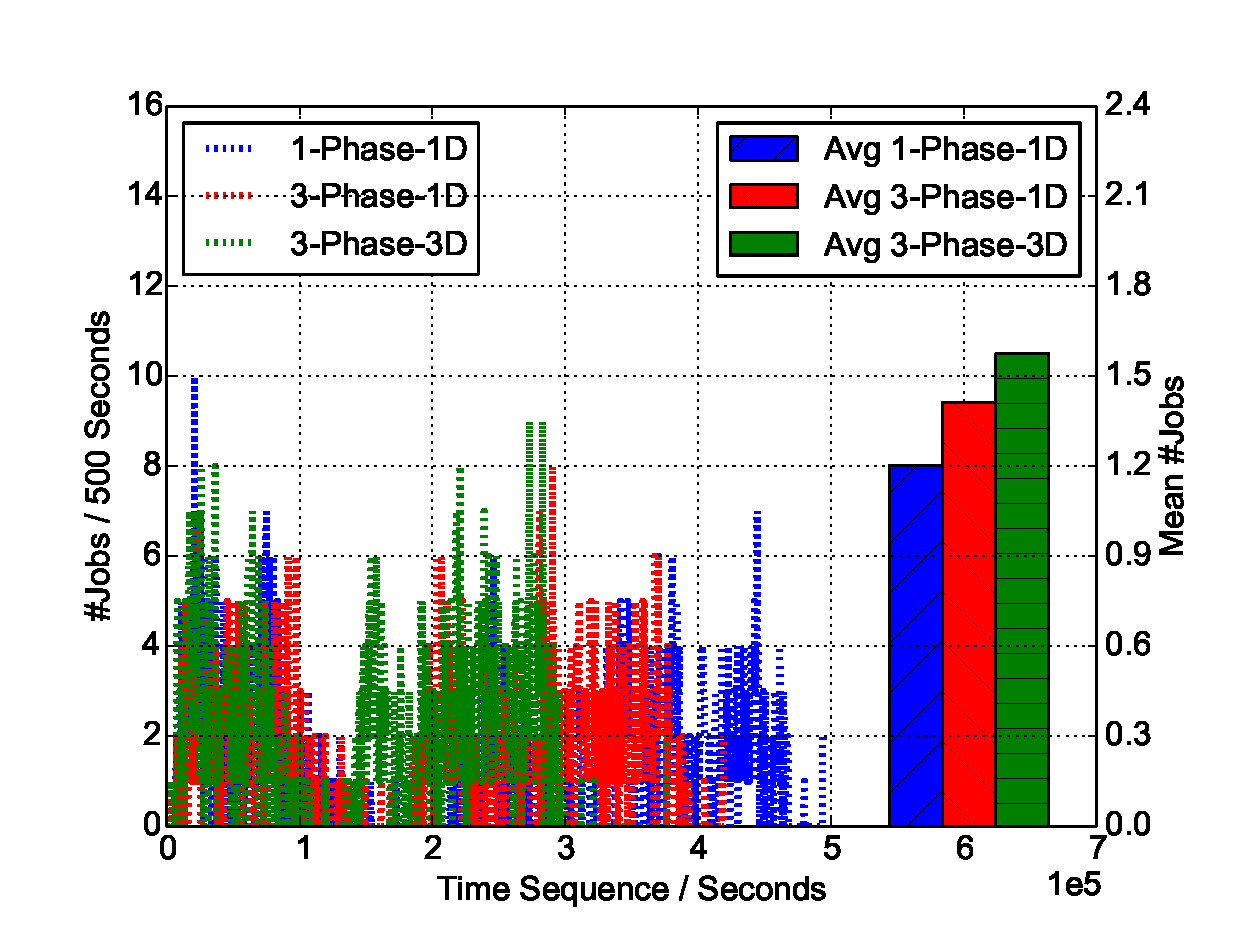
\includegraphics[width=3.2in]{3Pvs1PFigures/1000jobs_3p_vs_1p_throughput}
        \caption{System Throughput, 1 Phase Model vs. 3 Phase Model}
        \label{Fig:3Pvs1PThroughput}
\end{figure}


\begin{figure}[!t]
        \centering
        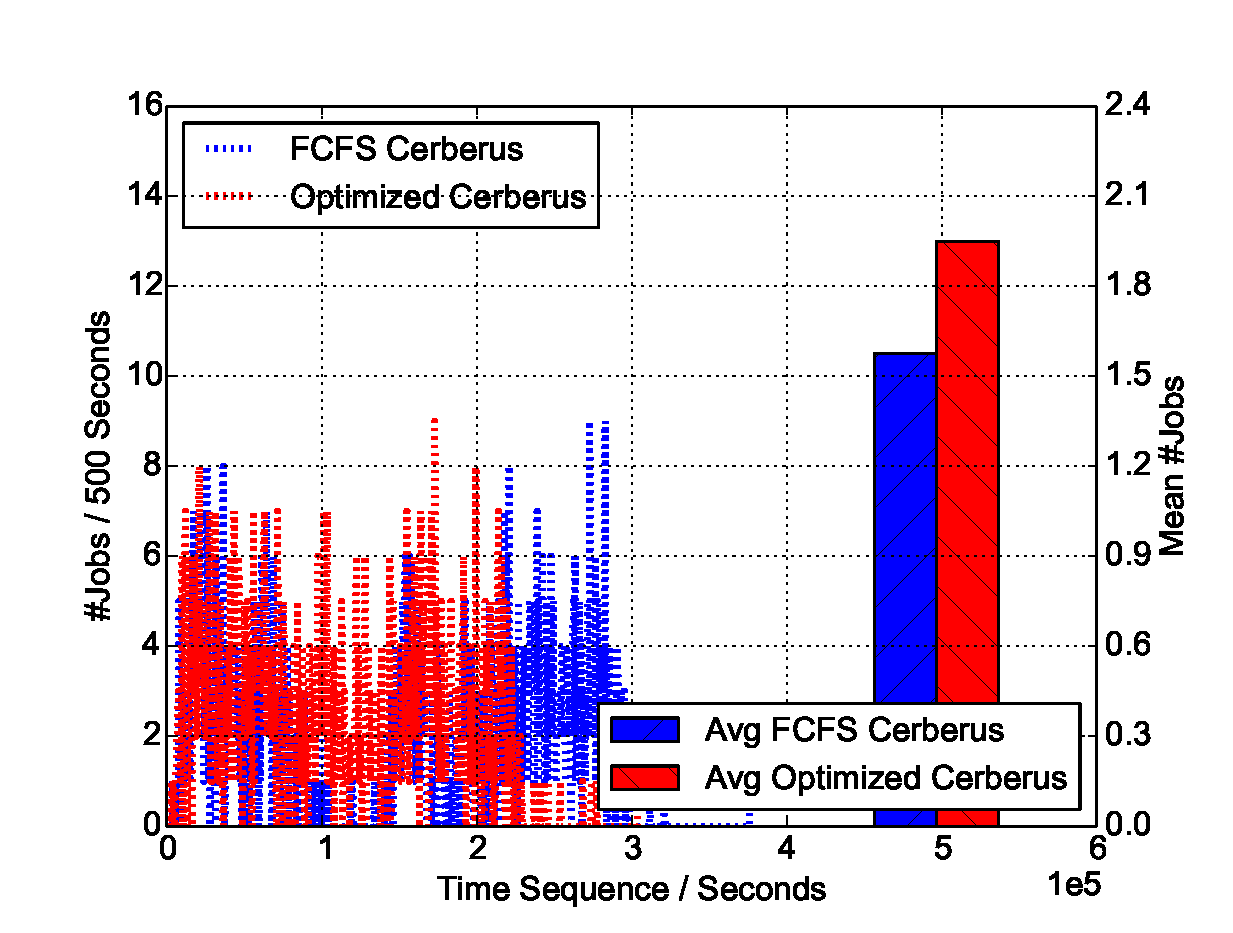
\includegraphics[width=3.2in]{DPvsFIFOFigures/1000jobs_dp_vs_fifo_throughput}
        \caption{System Throughput, Optimized Cerberus vs. FCFS Cerberus}
        \label{Fig:DPvsFIFOThroughput}
\end{figure}

%\begin{table}[!t] 
        %\renewcommand{\arraystretch}{1.3}
        %\caption{Time Consumption in Dynamic Programming}
        %\label{Tab:OptimizationTime}
        %\centering
        %\begin{tabular}{l|c|c|c}
                %\hline
                %Cerberus Version & FCFS & MaxT & MaxP \\
                %\hline
                %\hline
                %Simulation Time / seconds & 6.59 & 246.87 & 257.42 \\
                %Optimization Time / seconds & 0 & 241.11 & 251.75 \\
                %Total Number of Optimizations & 0 & 8702 & 9114 \\
                %\hline
        %\end{tabular}
%\end{table}

Table~\ref{Tab:OptimizationTime} demonstrate that our dynamic programming based
optimized Cerberus can schedule jobs online,
even though solving the optmization problem is thoretically NP-hard.
For MaxT Cerberus, it solved about 8400 Problems~\ref{Equ:MaxTransferData} and
Problem~\ref{Equ:MaxProduct} when scheduling 1185 jobs, taking less than 370 seconds.
MaxP Cerberus, similarly solves Problem~\ref{Equ:MaxTaskNumber} and
Problem~\ref{Equ:MaxProduct} in total 8220 times using less than 355 seconds.
The time of solving each optimization is about 0.04 seconds per time.

\begin{table}[!t] 
        \renewcommand{\arraystretch}{1.3}
        \caption{Time Consumption in Dynamic Programming}
        \label{Tab:OptimizationTime}
        \centering
        \begin{tabular}{l|c|c}
                \hline
                Optimization Policy Used & MaxT Cerberus & MaxP Cerberus \\
                \hline
                \hline
                Simulation Run Time / seconds & 375.55 & 362.40 \\
                Optimization Run Time / seconds & 364.62 & 354.39 \\
                Total Number of Optimizations & 8406 & 8220 \\
                \hline
        \end{tabular}
\end{table}



